\documentclass{beamer}

\usepackage{pgfplots}
\usepackage{appendixnumberbeamer}
\usepackage{multirow}
\usepackage[hang]{subfigure}

\usetheme{metropolis}

%Catalogue
%Viridis
\definecolor{viridis0}{rgb}{0.28, 0.13, 0.45}
\definecolor{viridis1}{rgb}{0.26, 0.24, 0.52}
\definecolor{viridis2}{rgb}{0.22, 0.34, 0.55}
\definecolor{viridis3}{rgb}{0.18, 0.44, 0.56}
\definecolor{viridis4}{rgb}{0.14, 0.52, 0.56}
\definecolor{viridis5}{rgb}{0.12, 0.61, 0.54}
\definecolor{viridis6}{rgb}{0.17, 0.69, 0.5}
\definecolor{viridis7}{rgb}{0.32, 0.77, 0.41}
\definecolor{viridis8}{rgb}{0.53, 0.83, 0.29}
\definecolor{viridis9}{rgb}{0.76, 0.88, 0.14}

%Catalogue
\definecolor{custom_one}{HTML}{00a0b0}
\definecolor{custom_two}{HTML}{eb6841}
\definecolor{custom_three}{HTML}{cc2a36}
\definecolor{custom_four}{HTML}{4f372d}
\definecolor{custom_five}{HTML}{183059}
\definecolor{custom_six}{HTML}{edc951}

\definecolor{custom_one}{HTML}{edc951}
\definecolor{custom_two}{HTML}{eb6841}
\definecolor{custom_three}{HTML}{cc2a36}
\definecolor{custom_four}{HTML}{4f372d}
\definecolor{custom_five}{HTML}{00a0b0}

\title{Human Age Prediction Based on Real and Simulated RR Intervals using Temporal Convolutional Neural Networks and Gaussian Processes}
\date{June 2, 2020 \hfill Supervisor: Krzysztof Bartoszek}
\author{Maximilian Pfundstein (maxpf364)\hfill Examiner: Oleg Sysoev}
\institute{Linköpings University}

\setbeamertemplate{frame footer}{Master Thesis (732A64)}

\begin{document}
    \maketitle
    
    \begin{frame}{Table of contents}
      \setbeamertemplate{section in toc}[sections numbered]
      \tableofcontents%[hideallsubsections]
    \end{frame}
    
    \section{Introduction}
    \begin{frame}{Introduction | Age Prediction}
        \begin{figure}[hbt]
        	\center
        	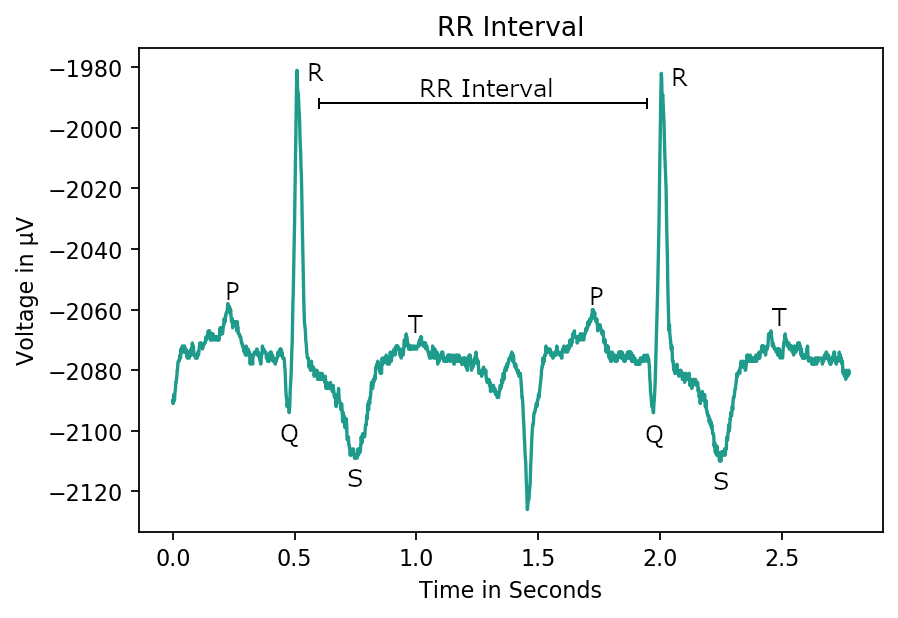
\includegraphics[width=1.0\textwidth]{img/rr-interval.png}
        	%\caption{}
        	\label{fig:rr}
        \end{figure}
    \end{frame}
    
    \begin{frame}{Introduction | Data Sets | Gdańsk}
        \begin{figure}[hbt]
        	\center
        	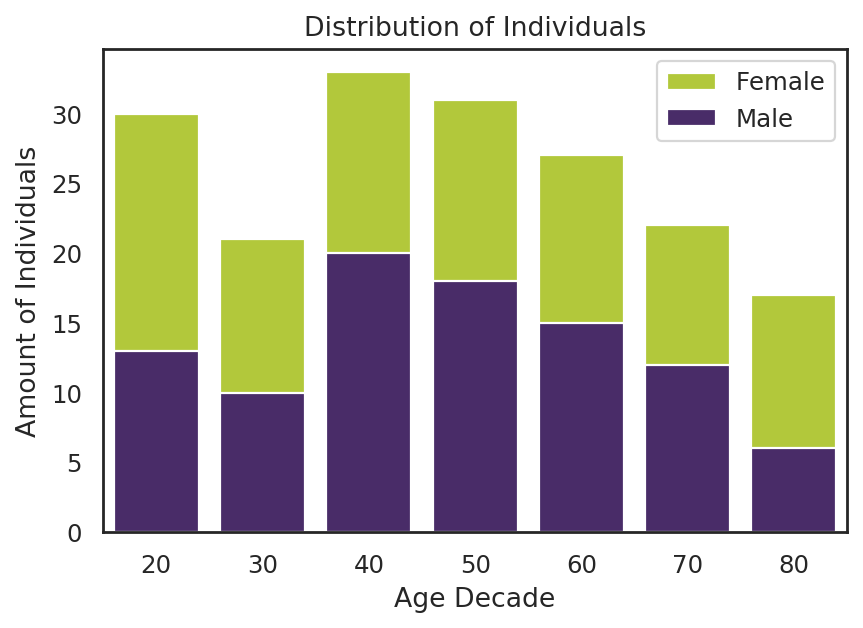
\includegraphics[width=1.0\textwidth]{img/gdansk-distribution-subjects.png}
        	%\caption{}
        	\label{fig:dist_gdansk}
        \end{figure}
    \end{frame}
    
    \begin{frame}{Introduction | Data Sets | PhysioNet}
        \begin{figure}[hbt]
        	\center
        	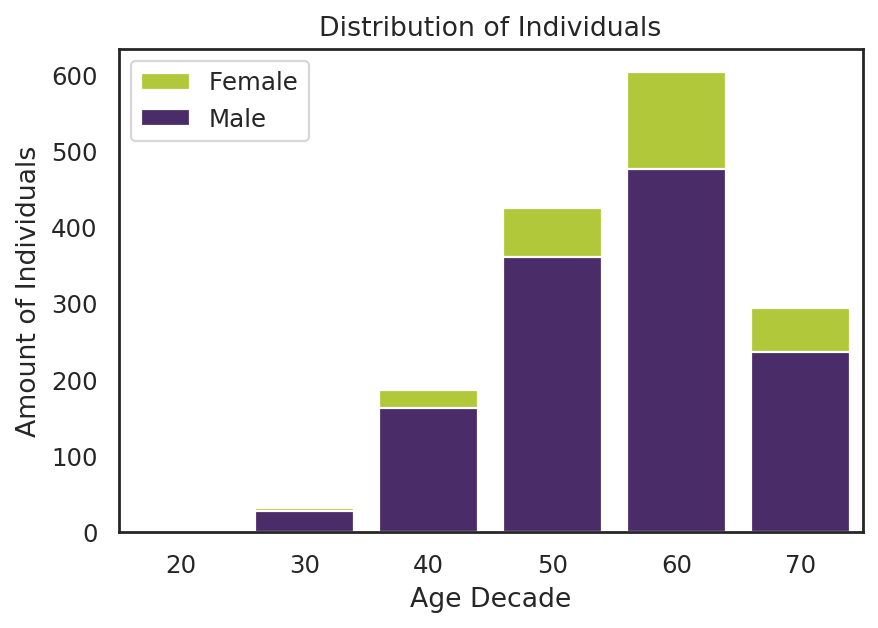
\includegraphics[width=1.0\textwidth]{img/physionet-distribution-subjects.png}
        	%\caption{}
        	\label{fig:dist_physionet}
        \end{figure}
    \end{frame}
    
    \begin{frame}{Introduction | Research Questions}
        \begin{itemize}
            \item Can the (cardiovascular) age of a person be predicted using recorded RR intervals and if yes, to which extend?
            \item Can RR intervals be simulated to generate training data, especially for deep learning models? How well does this work and does it improve the accuracy of the models?
        \end{itemize}
    \end{frame}
    
    \section{Data Cleaning}
    \begin{frame}{Data Cleaning | Linear Spline Interpolation}
        \begin{figure}[hbt]
        	\center
        	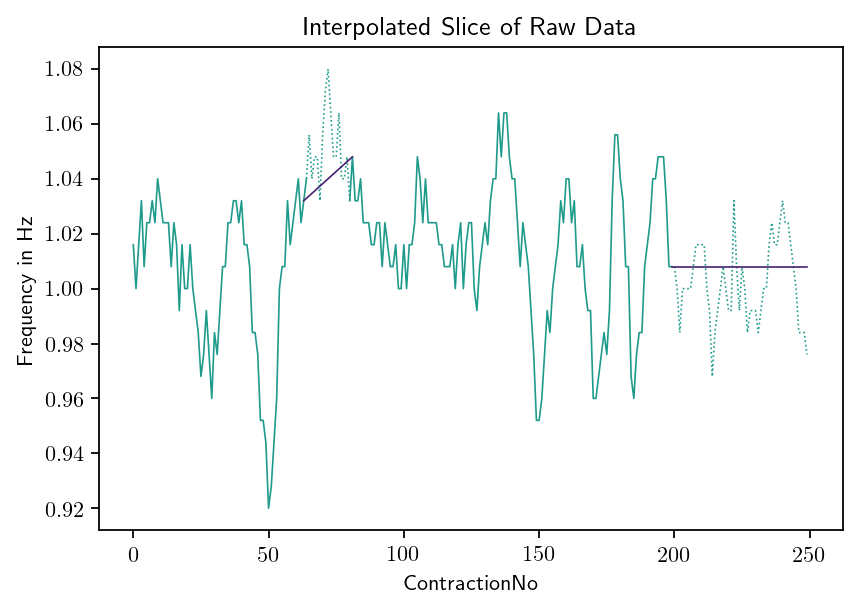
\includegraphics[width=1.0\textwidth]{img/slice_raw_data_linear_spline_interpolation.png}
        	%\caption{}
        	\label{fig:interpolation_and_padding}
        \end{figure}
    \end{frame}
    
    \begin{frame}{Data Cleaning | GP | Posterior Predictive Distribution}
        \begin{figure}[hbt]
        	\center
        	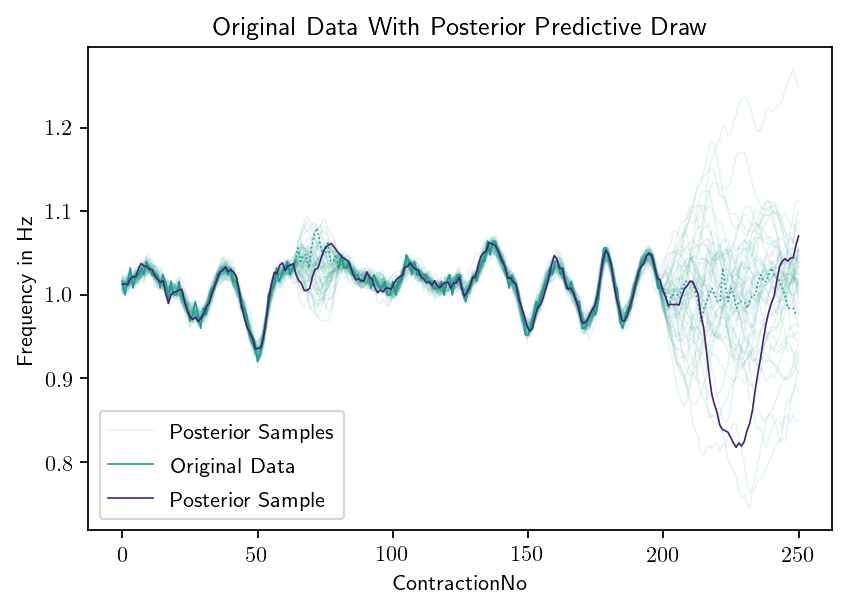
\includegraphics[width=1.0\textwidth]{img/gp_data_example_posterior_predictive.png}
        	%\caption{}
        	\label{fig:posterior_predictive_kernel}
        \end{figure}
    \end{frame}
    
        \begin{frame}{Data Cleaning | GP | Kernel Posterior Distributions}
        \begin{figure}[hbt]
        	\center
        	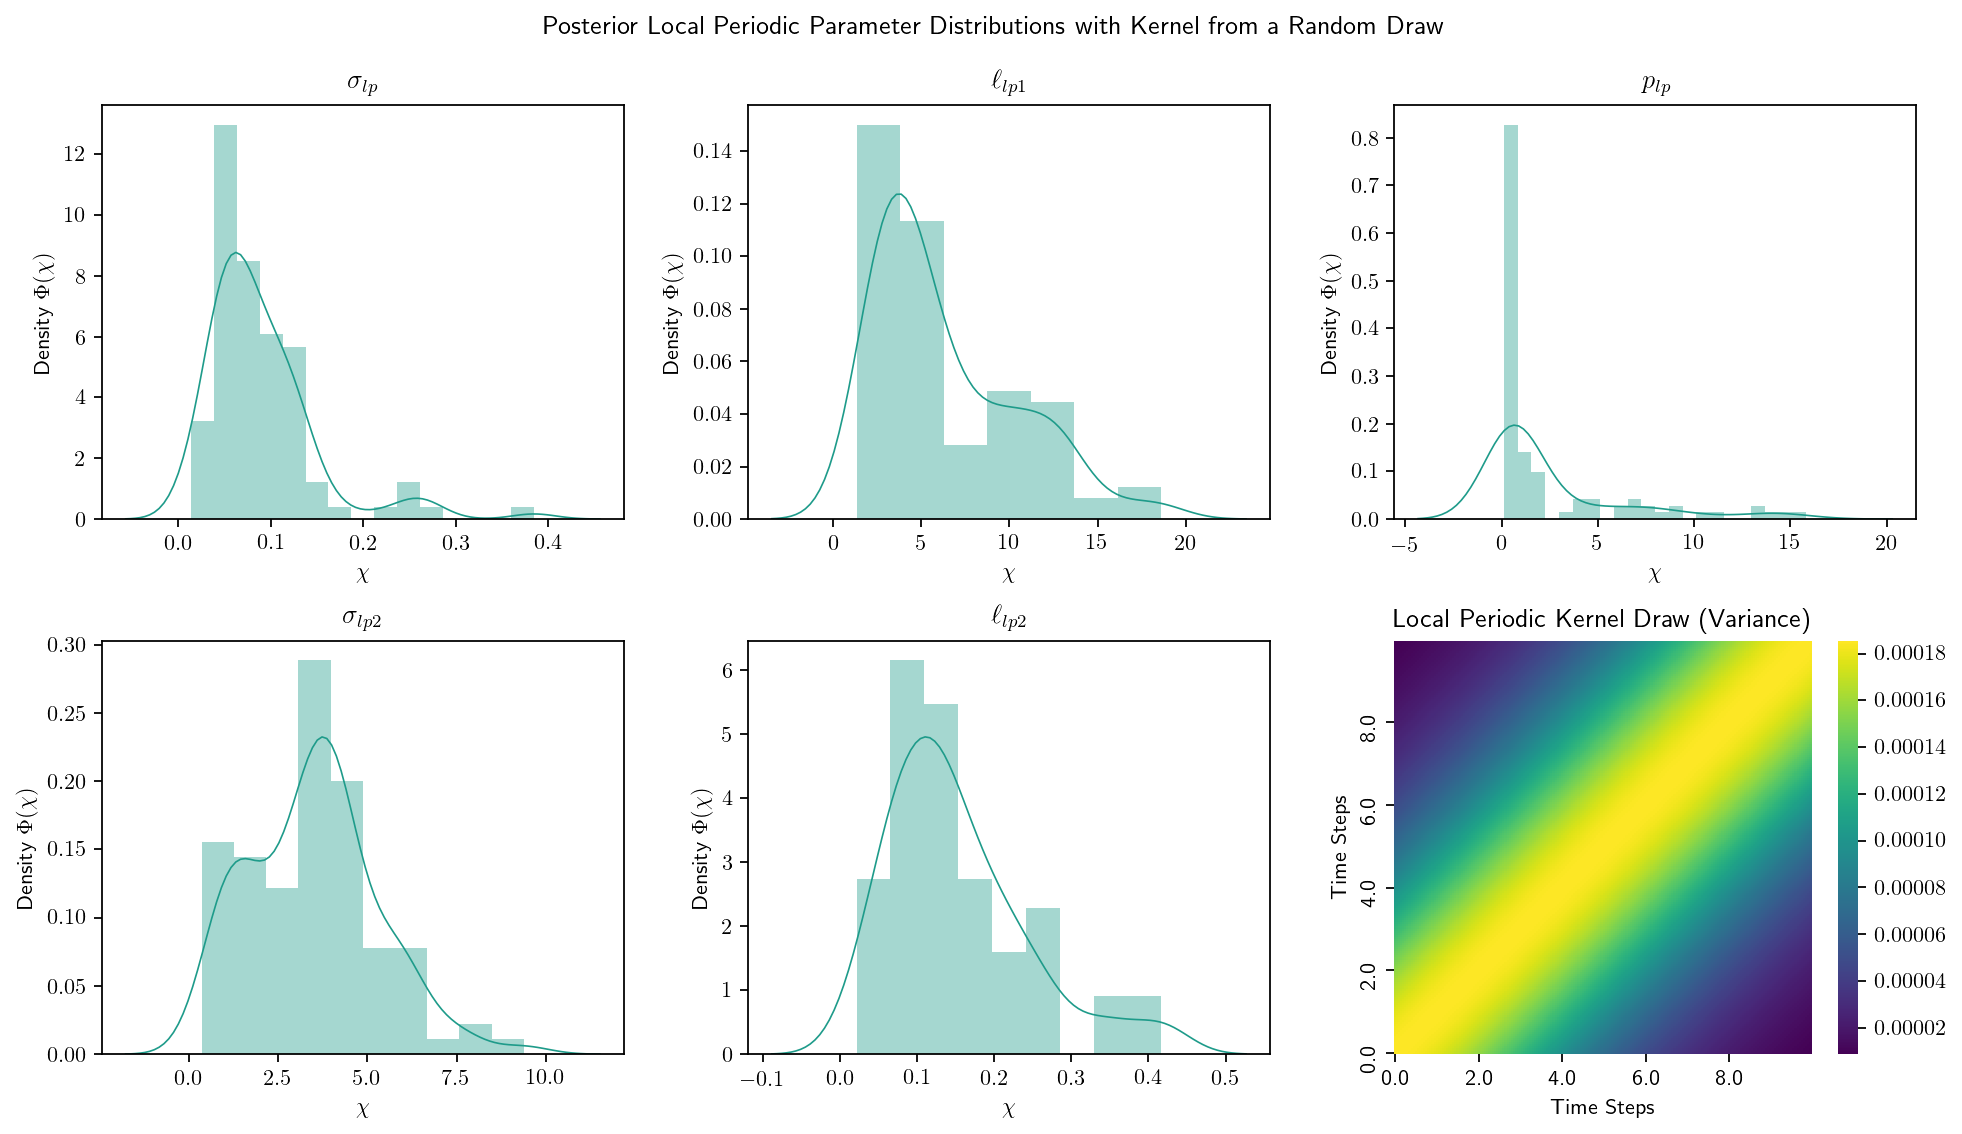
\includegraphics[width=1.0\textwidth]{img/gp_kernel_posterior_local_periodic_zoomed.png}
        	%\caption{}
        	\label{fig:posterior_predictive_kernel_local_periodic_zoomed}
        \end{figure}
    \end{frame}
    
    \section{Methods and Models}
    \begin{frame}{Methods and Models | Methods}
        \begin{itemize}
            \item \textit{complete} and \textit{constant}
            \item \textit{classification} and \textit{regression}
            \item Feature-Based:
            \begin{itemize}
                \item 33 features as used in a previous paper (\texttt{hrvanalysis})
                \item 3-fold cross validation with grid hyper-parameter search
                \item weighted loss
            \end{itemize}
            \item Deep-Learning:
            \begin{itemize}
                \item Dropout and early stopping for deep-learning
                \item weighted loss, under-sampling and over-sampling
            \end{itemize}
        \end{itemize}
    \end{frame}
    
    \begin{frame}{Methods and Models | Models}
        \begin{itemize}
            \item Naive Bayes
            \item Support Vector Machines
            \item Random Forest
            \item XGBoost
            \item DeepSleep-based
        \end{itemize}
    \end{frame}
    
    \begin{frame}{Methods and Models | DeepSleep}
        \begin{figure}[hbt]
        	\center
        	\includegraphics[width=0.5\textwidth]{img/deepsleep_part1.png}
        	%\caption{}
        	\label{fig:deepsleep}
        \end{figure}
    \end{frame}
    
    \begin{frame}{Methods and Models | DeepSleep}
        \begin{figure}[hbt]
        	\center
        	\includegraphics[width=0.7\textwidth]{img/deepsleep_part2.png}
        	%\caption{}
        	\label{fig:deepsleep}
        \end{figure}
    \end{frame}
    
    \section{Results}
    \begin{frame}{Results | Gdańsk}
    \begin{table}[h]
        \small
        \centering
        \begin{tabular}{lccr}
              & \textbf{Model} & \textbf{Method} & \textbf{Accuracy} \\
             \multicolumn{4}{@{}l}{} \\
             1. & Random Forest & complete regression & 37.83\% \\
             2. & Random Forest & constant classification & 32.43\% \\
             3. & DeepSleep-based & unweighted constant regression & 32.43\%
             \end{tabular}
        \caption{Results for the Gdańsk dataset. Baseline is 18.23\%.}
        \label{tab:results_gdansk}
    \end{table}
    \end{frame}

    \begin{frame}{Results | Physionet}
    \begin{table}[h]
        \small
        \centering
        \begin{tabular}{lccr}
              & \textbf{Model} & \textbf{Method} & \textbf{Accuracy} \\
             \multicolumn{4}{@{}l}{} \\
             1. & DeepSleep-based & unweighted constant classification & 42.58\% \\
             \end{tabular}
        \caption{Results for the Physionet dataset. Baseline is 39.14\%.}
        \label{tab:results_phyisonet}
    \end{table}
    \end{frame}
    
    \begin{frame}{Results | Simulated}
    \begin{table}[h]
        \small
        \centering
        \begin{tabular}{lccr}
              & \textbf{Model} & \textbf{Method} & \textbf{Accuracy} \\
             \multicolumn{4}{@{}l}{} \\
             1. & SVM & constant regression & 31.16\% \\
             2. & DeepSleep-based & oversampled constant regression & 29.51\% \\
             3. & DeepSleep-based & unweighted constant regression & 27.66\% 
             \end{tabular}
        \caption{Results for the Simulated dataset. Baseline is 18.23\%.}
        \label{tab:results_simulated}
    \end{table}
    \end{frame}
    
    \section{Discussion}
    \begin{frame}{Discussion | Results}
        \begin{itemize}
            \item Models perform better on the Gdańsk dataset
            \item Simulation and impurity handling did not improve the results
            \item The error distributions for all methods seem to be equal
            \item Results could be used for a very low number of classes
            \item Regression helps for deep learning, but not for feature-based models
            \item Precise age prediction based on RR intervals is \textbf{not} possible
        \end{itemize}
    \end{frame}
    
    \begin{frame}{Discussion | Results}
        \begin{figure}[hbt]
        	\center
        	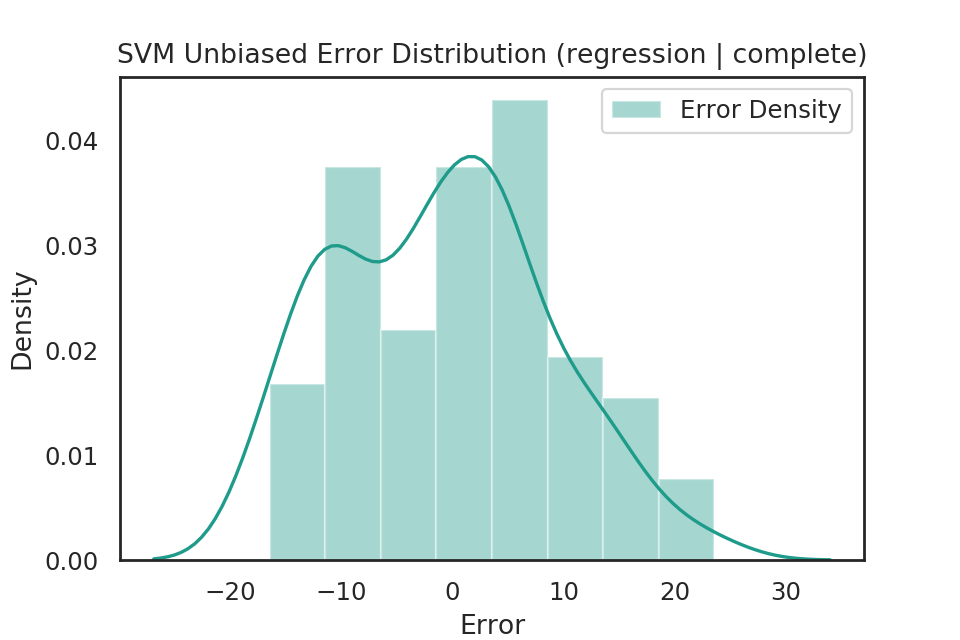
\includegraphics[width=1.0\textwidth]{img/physionet_svm_regression_complete_error_distribution_unbiased.png}
        	\caption{Physionet.}
        	\label{fig:example_error_distribution}
        \end{figure}
    \end{frame}
    
    \begin{frame}{Discussion | Findings}
        \begin{itemize}
            \item Tree-based models overfitted while still generalising best
            \item Weighting and oversampling gives worse results
            \item Deep learning scales better than most feature-based models
            \item Loss and accuracy during training for classification and regression
        \end{itemize}
    \end{frame}
    
    \begin{frame}{Discussion | Findings}
        \begin{figure}[!hbt]
            \makebox[\linewidth][c]{
        	\centering
        	\subfigure[Loss]{\label{fig:original_gdansk_sleepnet_classification_complete_none_unweighted_loss}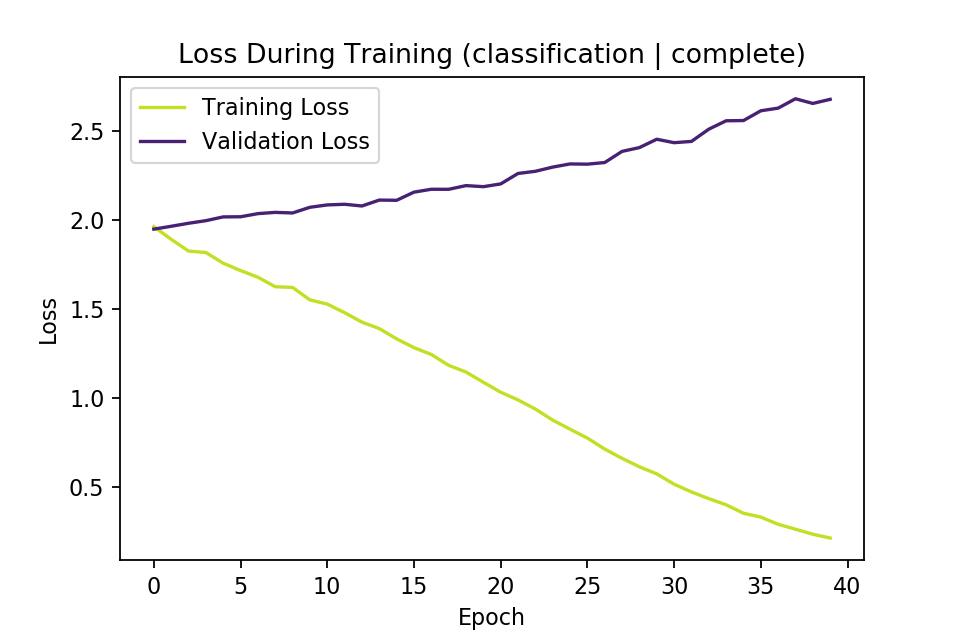
\includegraphics[width=0.6\textwidth]{img/original_gdansk_sleepnet_classification_complete_none_unweighted_loss.png}}
        	\subfigure[Accuracy]{\label{fig:original_gdansk_sleepnet_classification_complete_none_unweighted_accuracy}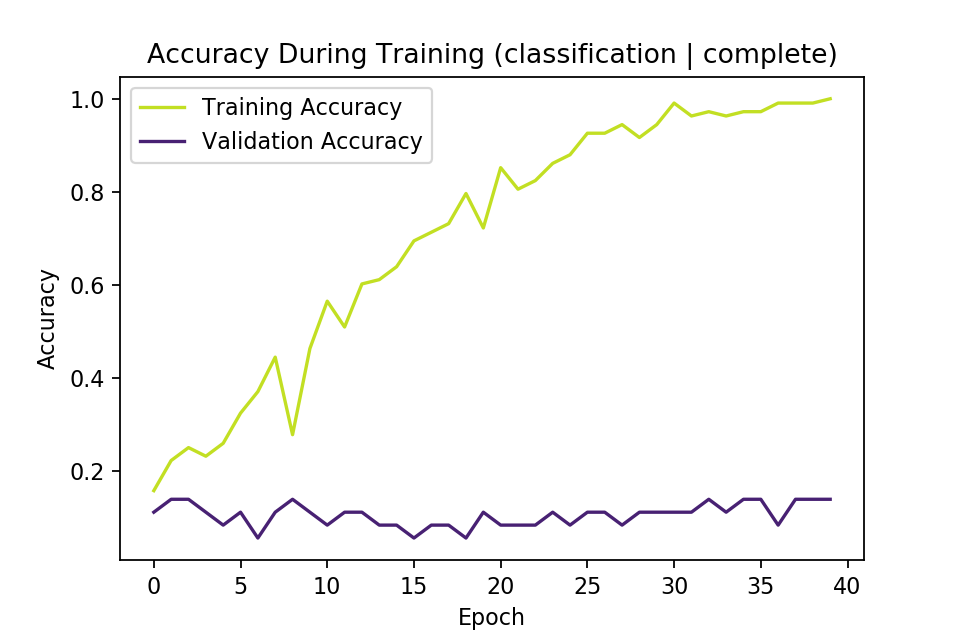
\includegraphics[width=0.6\textwidth]{img/original_gdansk_sleepnet_classification_complete_none_unweighted_accuracy.png}}
        	}
        	\caption{\textcolor{viridis9}{\textbf{Training}} and \textcolor{viridis0}{\textbf{validation}} loss and accuracy for DeepSleep performing standard complete classification.}
        \end{figure}
    \end{frame}
    
    \begin{frame}{Discussion | Findings}
        \begin{figure}[!hbt]
            \makebox[\linewidth][c]{
        	\centering
        	\subfigure[Loss]{\label{fig:original_gdansk_sleepnet_regression_constant_oversample_loss}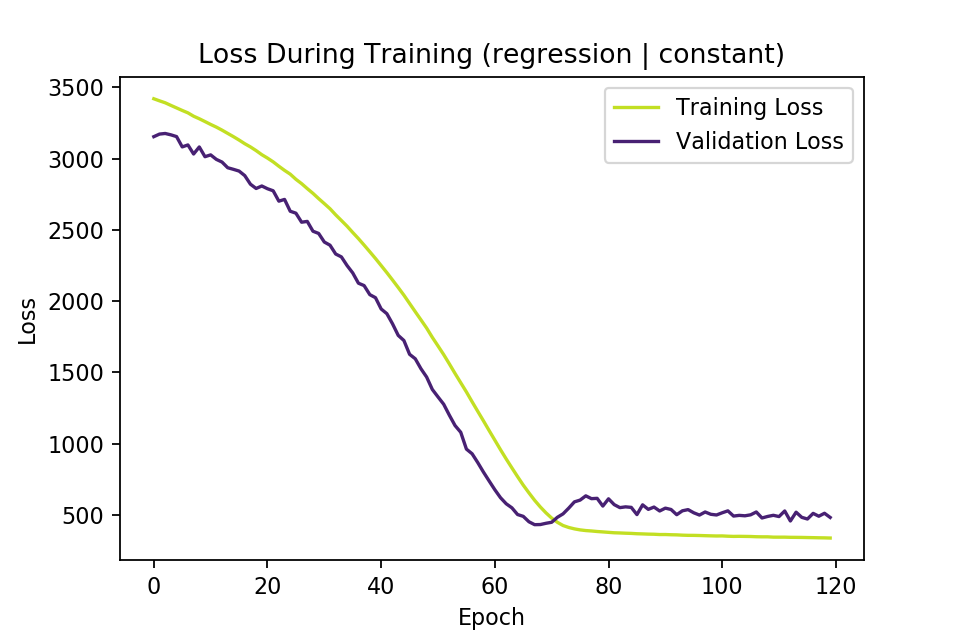
\includegraphics[width=0.6\textwidth]{img/original_gdansk_sleepnet_regression_constant_oversample_loss.png}}
        	\subfigure[Accuracy]{\label{fig:original_gdansk_sleepnet_regression_constant_oversample_accuracy}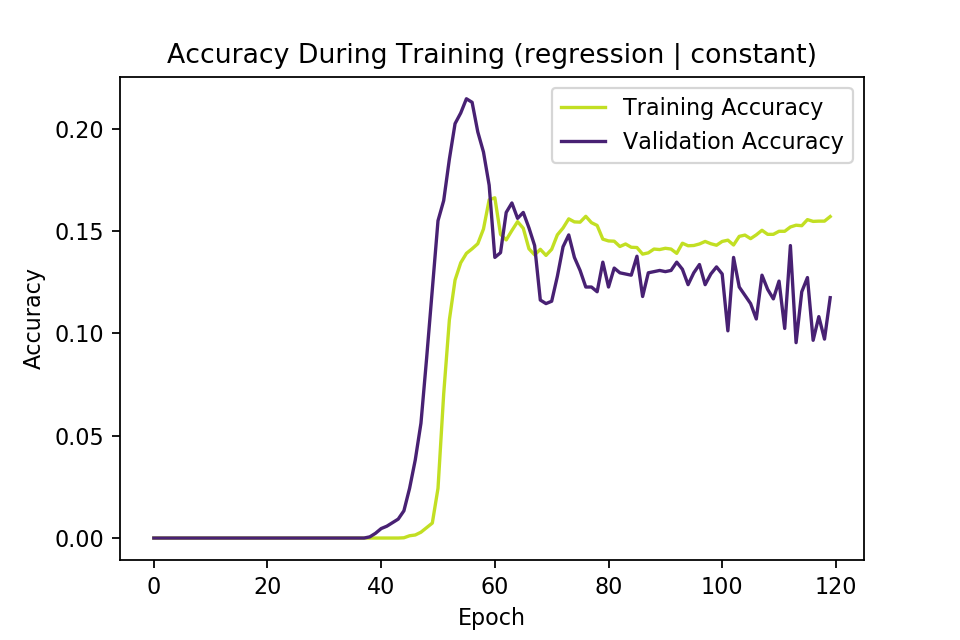
\includegraphics[width=0.6\textwidth]{img/original_gdansk_sleepnet_regression_constant_oversample_accuracy.png}}
        	}
        	\caption{\textcolor{viridis9}{\textbf{Training}} and \textcolor{viridis0}{\textbf{validation}} loss and accuracy for DeepSleep performing oversampled constant regression.}
        \end{figure}
    \end{frame}
    
    \begin{frame}{Discussion | Validity}
        \begin{itemize}
            \item Comparison with other papers
            \item \cite{threeclassclassification} report accuracies of $\sim$ 70\% for 3 classes
            \item \cite{patternshrd} report accuracies over 90\% for 7 classes
            \begin{itemize}
                \item No test dataset
                \item Their SVM chose $C = 1.0$ and $\gamma = 0.2$
                \item Probably overfitted to the training data
            \end{itemize}
        \end{itemize}
    \end{frame}
    
    \section{Conclusions \& Outlook}
    \begin{frame}{Conclusions}
        \begin{itemize}
            \item Cardiovascular age prediction based on RR intervals is hard
            \item Linear Spline Interpolation works sufficiently well
            \begin{itemize}
                \item Maybe due to the fact that the information we seek is not embedded in the signal
            \end{itemize}
        \end{itemize}
    \end{frame}
    
    \begin{frame}{Outlook}
        \begin{itemize}
            \item Analyse simulation on a signal where information is obviously embedded
            \item Use the raw signal no embed for information
            \begin{itemize}
                \item e.g. P, Q, S and T denotations
            \end{itemize}
        \end{itemize}
    \end{frame}
    
    \appendix
    
    \begin{frame}[standout]{}
        \center Appendix
    \end{frame}
    
    \begin{frame}[allowframebreaks]{References}
    
      \bibliography{literature.bib}
      \bibliographystyle{apalike}
    
    \end{frame}
    
\end{document}